\documentclass[12pt,answers]{exam}


\usepackage{graphicx}
\usepackage{amsmath}
\usepackage{color}
\usepackage{amssymb}
% \usepackage{setspace}
% \usepackage{epstopdf}
% \usepackage{empheq}
\usepackage{csquotes} % \textcquote
\usepackage{parskip}
% \setlength{\marginparwidth}{2cm}
% \usepackage{easyReview} % \alert, \highlight, \remove, \add, \replace, \comment
% \usepackage{subcaption}
% \usepackage[letterpaper]{geometry}
% \usepackage[definethebibliography]{easybib}
\usepackage{float}
\renewcommand{\solutiontitle}{\noindent\textbf{Authors Reply:}\par\noindent}

\usepackage{tikz}
\tikzstyle{block} = [rectangle, minimum width=2cm, minimum height=1cm,text centered, draw=black]
\tikzstyle{block_1} = [rectangle, minimum width=2cm, minimum height=1cm,text centered, draw=black, fill=blue!5]
\tikzstyle{block_2} = [rectangle, minimum width=2cm, minimum height=1cm,text centered, draw=black, fill=red!5]
\tikzstyle{arrow} = [thick,->,>=stealth]
\tikzstyle{arrow_2} = [very thick,->,>=stealth]
\tikzstyle{arrow_3} = [thick,->,>=stealth,dashed]
\tikzstyle{pfr} = [cylinder, draw, minimum height=4cm, minimum width=1cm, shape aspect=1, shape border rotate=180]
\usetikzlibrary{shapes.geometric}

\begin{document}

\section*{Common concerns}

Before addressing each reviewer's comments individually, we would like to discuss two common concerns raised by multiple reviewers: the modeling approach and the parameter sensitivity analysis.

\subsection*{Modeling approach}

We recognize that the initial submission provided a limited explanation of the original model. To address this, we have expanded our explanation both here and in the updated manuscript, resulting in a more general model while keeping its changes minimal. These revisions directly address the reviewers' concerns and remain consistent with the intent of the initial model.

Nevertheless, our work aims to establish a foundation for future research in this area by developing a modeling and control strategy within a general framework. This framework is designed to encompass key features of real-world systems, rather than focusing on a model tailored to a specific system. 

For the axial dispersion tubular reactor presented in Fig.~\ref{fig:reactor}, the molar balance equation may be written for the reactant concentration, $C_A$, as follows:

\begin{figure}[!htbp]
    \centering
    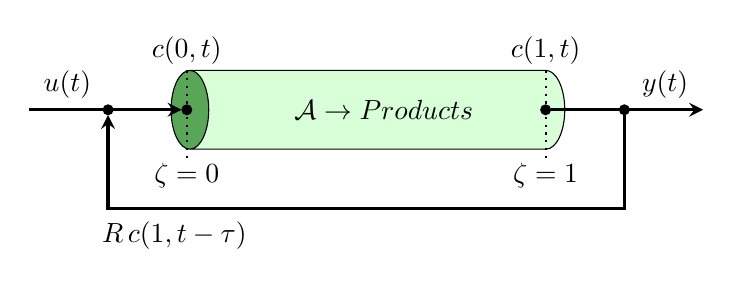
\begin{tikzpicture}
        \node (pfr) [cylinder, draw, minimum height=5cm, minimum width=1cm, shape aspect=1, shape border rotate=180, cylinder uses custom fill, cylinder end fill=green!30!gray, cylinder body fill=green!15] {$\mathcal{A} \rightarrow {Products}$};
        \node (pfr_inlet) [circle, left of=pfr, xshift=-1.5cm, fill=black, draw, inner sep=0pt, minimum size=0.25cm, scale=0.5] {};
        \node (pfr_outlet) [circle, at={(pfr.east)}, shift={(-0.25cm,0)}, fill=black, draw, inner sep=0pt, minimum size=0.25cm, scale=0.5] {};
        \node (recycle_right) [circle, right of=pfr_outlet, fill=black, draw, inner sep=0pt, minimum size=0.25cm, scale=0.5] {};
        \node (recycle_left) [circle, left of=pfr_inlet, fill=black, draw, inner sep=0pt, minimum size=0.25cm, scale=0.5] {};
    
        \draw[dotted, thick] ([yshift=0.5cm]pfr_inlet.center) -- node[at end, below, yshift=0.1cm] {$\zeta = 0$} ([yshift=-0.65cm]pfr_inlet.center);
        \draw[dotted, thick] ([yshift=0.5cm]pfr_outlet.center) -- node[at end, below, yshift=0.1cm] {$\zeta = 1$} ([yshift=-0.65cm]pfr_outlet.center);
    
        \node[below of=recycle_left, node distance=1.3cm, anchor=north west, xshift=-0.2cm] {$R \, c(1, t-\tau)$};
        \node[above of=pfr_inlet, node distance=0.75cm,] {$c(0, t)$};
        \node[above of=pfr_outlet, node distance=0.75cm,] {$c(1, t)$};
        
        \draw [arrow_2] (pfr_outlet) -- node[near end, above] {$y(t)$} ++(2,0);
        \draw [arrow_2] (pfr_inlet) ++(-2,0) coordinate(start) -- node[near start, above] {$u(t)$} (pfr_inlet);
        \draw [arrow_2] (recycle_right) -- ++(0,-1.25) -| (recycle_left);
        
    \end{tikzpicture}
    \caption{Axial tubular reactor with recycle stream.}
    \label{fig:reactor_scheme}
\end{figure}

\begin{equation}
    \frac{\partial C_A}{\partial t} = D \frac{\partial^2 C_A}{\partial \zeta^2} - v \frac{\partial C_A}{\partial \zeta} - r(C_A)
\end{equation}

where $r(C_A)$ is the reaction rate by which the reactant is consumed. Considering this term can be non-linear, the model can be linearized around the steady-state followed by replacing the state of the system with deviation from the steady-state concentration. This will result in the following equation:

\begin{equation}
    \frac{\partial \epsilon}{\partial t} = D \frac{\partial^2 \epsilon}{\partial \zeta^2} - v \frac{\partial \epsilon}{\partial \zeta} - \left. \frac{\partial r(C_A)}{\partial C_A} \right|_{C_{A, ss}} \epsilon
\end{equation}

Here, $\epsilon \equiv C_A - C_{A, ss}$ is the deviation from the steady-state concentration, and $C_{A, ss}$ is the steady-state concentration of the reactant. The model given at this point, although linear, sets a general framework for model-based control strategies of a wide range of infinite-dimensional convection-diffusion-reaction systems in chemical engineering process and dynamics around their steady-state.

The assumptions made in the model are that the parameters of the system are constant and thus, the states of the system are not affected by changes in system's pressure or temperature. The authors acknowledge that the model will be more realistic if the temperature dependence of the reaction rates is included. In fact, addressing temperature dependence is the focus of our ongoing research and represents a natural extension of this work. We anticipate presenting these advancements in future submissions to this journal. Nevertheless, as mentioned above, the primary goal here is to establish a general framework, leaving more specific and physically significant models for subsequent studies.

In addition to the concerns related to the applicability of the model, the choice of positive reaction term is also explained in this section along with stability analysis. The stability analysis of the system in the vicinity of the steady state has been one of the first things of our interest. While no isothermal reactor can technically be exponentially unstable due to the finite amount of reactant available, the steady state of the system can be unstable in the vicinity of the steady state, meaning that a deviation from the steady state may draw the system to a different steady state, resulting in completely different model dynamics than the one used to design and control the system for optimal operation.

Performing the eigenvalue analysis of the system, we have observed that a system may have unstable steady-state only when the reaction term coefficient $\frac{\partial r(C_A)}{\partial C_A}$ is positive. Though an uncommon scenario, this may happen in the case of autocatalytic reactions, enzyme-catalyzed reactions, reactions that incorporate inhibition mechanisms, etc. Although the proposed controller can also stabilize an already stable system in an optimal manner, a positive reaction term is selected to demonstrate the ability of the proposed controller to stabilize a system which is mathematically unstable, rather than focusing on a physically significant model. This has to be included within the general framework of the controller proposed in this work as it becomes more significant when the work is extended to more complex systems where instability becomes a common issue.


\subsection*{Parameter sensitivity analysis}



\newpage

\section*{Reviewer 1}

The comments of Reviewer 1, along with our responses to each comment, are included below:

\begin{quote}
    \textquote{This work presents a boundary optimal control strategy for axial tubular reactors with first-order irreversible chemical reaction incorporating a delayed recycle stream. The mathematical description takes the form of a system of coupled parabolic and hyperbolic PDEs. An infinite-dimensional approach is applied to derive a linear quadratic regulator with and without observer. Numerical studies show that the proposed controller is able to stabilize the system. The manuscript is clear and well written and addresses a challenging control problem in chemical engineering. The following comments and suggestions may improve the presentation so that it is considered for publication.}
\end{quote}

\begin{questions}

    \question Page 3 - \textquote{Many chemical, petrochemical, and biochemical unit operation processes are modelled as
    distributed parameter systems (DPS).}

    A few specific examples of these chemical processes would help to motivate the problem this paper addresses

    \begin{solutionorbox}
        Examples have been added to the introduction and the manuscript has been revised accordingly.
    \end{solutionorbox}

    \question Page 5 - \textquote{PIDEs}

    - What does PIDEs stand for?

    \begin{solutionorbox}
        Thanks for pointing this out. The acronym should have been defined in the manuscript. It stands for Partial Integro Differential Equations. The manuscript has been revised accordingly.
    \end{solutionorbox}


    \question Page 5 - \textquote{a configuration common in industrial processes}

    - Examples of these processes would illustrate the need and motivation to address the associated
    control problem

    \begin{solutionorbox}
        Examples have been added to the introduction and the manuscript has been revised accordingly.
    \end{solutionorbox}


    \question Page 6 - \textquote{The resulting PDE that describes the reactor model is given by:}

    - I suggest to specify the assumptions leading to the reactor model, like isothermal operation,
    constant properties, constant pressure, ...

    \begin{solutionorbox}
        We have assumed that the parameters of the system are constant and thus, the states of the system are not affected by changes in system's pressure or temperature. The manuscript has been updated to include more detailed explanation in this regard.
    \end{solutionorbox}


    \question Page 7 - Eq (2)

    - What is the physical meaning of the manipulated variable $u(t)$?

    \begin{solutionorbox}
        It is of the same nature as the system's states, i.e. the manipulated variable $u(t)$ may be seen as either the product concentration or as its deviation from the steady-state concentration in the reactor feed stream. The manuscript has been updated to address this point.
    \end{solutionorbox}


    \question Page 7 - \textquote{ $x_2(\zeta, t)$ is introduced as a new state variable to account for the concentration along the recycle stream}

    - Why is $x_2$ a function of $\zeta$ ? How does $x_2$ change across the recycle? What kind of law does it follow? To me, it seems like $x_2$ only changes with respect to time

    \begin{solutionorbox}
        We have assumed that along the recycle stream, the flow of the reactant belongs to the class of pure transport PDEs. This is the case when diffusion term and reaction term become negligible compared to the convective term, and the state variable $x_2$ is merely being transported along the recycle stream. Nevertheless, this still means that $x_2$ is a function of $\zeta$ and $t$. Concentration profile along the recycle stream has not been presented in the original submission as we believe it is not the focus of this work. However, for the reviewer's reference, it is included here in the response as shown in Fig.~\ref{fig:x2}.
    \end{solutionorbox}

\begin{figure}[H]
    \centering
    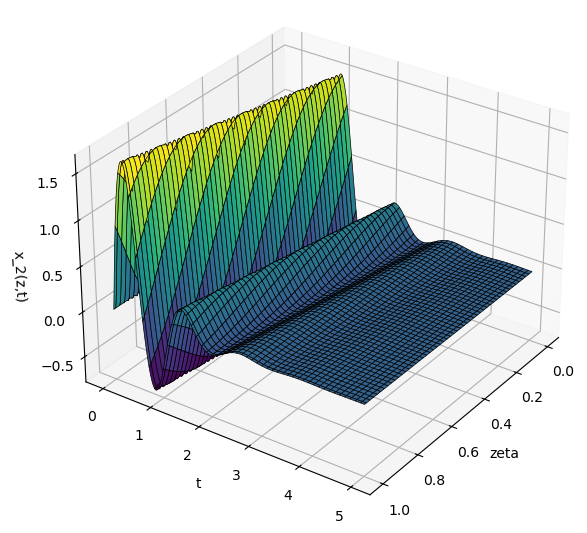
\includegraphics[width=0.65\textwidth]{x2_vs_z.png}
    \caption{Concentration profile along the recycle stream}
    \label{fig:x2}
\end{figure}

    \question Page 8 - Eq (5)
    
    - Please make a distinction between the symbol for domain and for diffusivity to avoid confusion

    \begin{solutionorbox}
        Thanks for mentioning this. We have replaced the symbol for the domain with $\mathcal{D}$ to avoid confusion. The manuscript has been updated accordingly.
    \end{solutionorbox}


    \question Page 12 - Riesz-spectral operator $\mathfrak{A}$

    - Although a rigorous proof is not necessary, it would be good if the authors explain why $\mathfrak{A}$ is a Riesz-spectral operator. I guess its eigenvalues and eigenfunctions satisfy the requirements, like having multiplicity one and forming a Riesz basis, respectively.

    \begin{solutionorbox}
        That, along woth the fact that the obtained set of eigenfunctions for $\mathfrak{A}$ and $\mathfrak{A}^*$ seem to form a bi-orthogonal basis that can successfully span the state space, is the reason behind this statement. It is worth mentioning that as the result of the nature of boundary conditions, this can not be analytically proven. However, once the spectrum for the system generator and its adjoint is obtained and the eigenfunctions are properly scaled, we observe that the aforementioned properties are satisfied. To be more specific, the inner products of $\phi_i$ and $\psi_j$ gives $\delta_{i,j}$, and every arbitrary function that satisfies the domain may be expressed as a linear combination of the given bi-orthogonal basis. In the manuscript, we have avoided going into the details to keep the flow of the paper.
    \end{solutionorbox}


    \question Page 12 - $\mathfrak{R}$ being positive semi-definite operator

    - Should $\mathfrak{R}$ be self-adjoint and coercive?

    \begin{solutionorbox}
        Yes. According to \cite{curtainbook} for the infinite-dimensional LQR problem on the infinite-time interval, operator $\mathfrak{R}$ should be self-adjoint and coercive, which is a better way to address the operator compared to self-adjoint and positive semi-definite. The manuscript has been updated accordingly.
    \end{solutionorbox}


    \question Page 12 - The LQR problem

    - Is Problem 12 well-posed, does J have a finite value for at least one u?

    \begin{solutionorbox}
        Yes, the proposed infinite-time LQR problem is well-posed, i.e. for at least one input trajectory $u(t)$, the cost function $J$ has a finite value. The stabilizing input trajectory obtained in the manuscript is an example. % check with stevan
    \end{solutionorbox}


    \question Page 18 - unstable dynamics of the model

    - Why is the zero-input response considered unstable? Is it a qualitatively assessment? What is the physical meaning of Figure 9?

    \begin{solutionorbox}
        The open-loop system being unstable is the result of the reaction term being positive, which opens up an opportunity for deeper analysis to explore underlying mechanisms and implications. We basically picked the positive reaction term to demonstrate the ability of the proposed controller to stabilize a mathematically unstable system. However, the physical significance of the system described by such a model may be further explored by focusing on the reaction kinetics and first principle modeling. 
        
        The reaction kinetics can be seen in two ways: first, the state of the system being described by the reactant concentration, and second, the state being described by the product concentration. 

    \begin{enumerate}
        \item  $x_1 = C_A$: In this case, the reaction is either a first-order reaction, or the reaction rate is a non-linear function of the state. In the latter case, the non-linear system can be linearized around the steady-state followed by replacing the state of the system with deviation from the steady-state concentration. In the obtained model, the reaction constant parameter $k_r$ shall be negative as long as the state of the system is the reactant concentration. This is because the reactant is being conmsumed over time.
        \item $x_1 = C_B$: In this case, the reaction rate is generally a nonlinear function of the product concentration. Same as previous, the system can be linearized around the steady-state followed by replacing the state of the system with deviation from the steady-state concentration. In the obtained model, the reaction constant parameter $k_r$ shall be positive as long as the state of the system is the product concentration. Unlike the previous case, this is because the product is being generated over time. In a rare case, such as auto-catalytic reactions where the reactant is available in excess, the reaction rate can be directly expressed as a linear function of the product concentration as long as the excess reactant assumption holds.
    \end{enumerate}
    
    Since the source of instability according to the above, is merely the accumulation of the products, it is rare to have an unstable system in practice. Because even if the rate law determines the rate of product accumulation increases with the product concentration, the system will eventually run out of reactants and the reaction will stop. In fact, most unstable reaction systems are due to the temperature dependence of the reaction rates, resulting in runaway reactions.
    
    Nevertheless, the key contribution of this work lies in introducing a control strategy based on a novel approach to address the problem of intrinsic delay imposed by the recycle stream. This strategy forms a foundation for future research and development for the general case of second order parabolic PDE systems, rather than focusing solely on a model with realistic physical significance. As mentioned earlier, the motivation behind the choice of positive reaction term in the model is to demonstrate the ability of the proposed controller to stabilize a system which is mathematically unstable, at least in the vicinity of its steady state where the linearization is valid. 
    
    We have adjusted the manuscript briefly to better explain what it means for the system to be unstable in this context. Future works will extend the same control and modeling strategy to address physically significant unstable reaction systems by including the assumption of temperature dependence for the reaction rates.

    \end{solutionorbox}


    \question Page 18 - \textquote{The goal is to stabilize the system using an optimal control strategy}

    - What are the values of matrices Q and R in the objective function?

    \begin{solutionorbox}
        Thanks for pointing this out. The values for operators $\mathfrak{Q}$ and $\mathfrak{Q}$ in the objective function were not explicitly mentioned in the manuscript. These values are chosen as $\mathfrak{Q} = 0.05 \times \mathfrak{I}$ and $\mathfrak{R} = 50$, where $\mathfrak{I}$ is the identity operator of the same size as $\mathfrak{A}$. The manuscript has been updated accordingly.
    \end{solutionorbox}


    \question Page 18 - \textquote{The goal is to stabilize the system using an optimal control strategy}

    - Are x deviation variables? What is the setpoint?

    \begin{solutionorbox}
        In addition to our reply to question 11, since the reactionterm is positive in the proposed PDE, the state of the system may be seen as either the product concentration or as its deviation from the steady-state concentration. The setpoint will be either zero or the steady-state concentration of the product, respectively. Again, the goal of this work is to establish an optimal controller strategy to stabilize a system described by the proposed model, rather than tracking a physically significant setpoint.
    \end{solutionorbox}


    \question Page 20 - \textquote{Both optimal feedback gains are able to successfully stabilize the system within finite time horizon.}

    - It would be interesting to see how the delay time affects the stabilizing capabilities of the feedback regulator. What would happen a shorter and larger values of $\tau$

    \begin{solutionorbox}
        It is indeed interesting to see the effect of system parameters (e.g. recycle delay, $\tau$, or recycle ratio, $R$) on the spectrum of the system as well as the controller performance. We have explored numerous scenarios in the numerical simulations and observed that increasing the recycle ratio, $R$, or the recycle delay, $\tau$, may lead to more challenging control problems. However, the proposed controller is able to stabilize the system for a wide range of system parameters with exactly the same strategy. Since exploring different system parameters appeared to add no direct significant value to the main contribution of the paper, we have decided to keep the focus on the proposed control strategy in the original manuscript. Nevertheless, if the reviewer finds it necessary, we can include a new plot profile in the revised manuscript where the closed-loop system state is plotted for one or two different values of $\tau$ and/or $R$.
    \end{solutionorbox}


    \question Page 26 - \textquote{The proposed framework may be extended to more complex diffusion-convection reactor configurations, such as non-isothermal reactors}

    - Can this framework be applied to reaction systems described with more complex and highly nonlinear reaction kinetics?

    \begin{solutionorbox}
        Yes, it can. The general approach would be the same as the one presented in \cite{khatibi2021model}, where they assumed the reaction constants to be exponential functions of the temperature. The same approach can be applied to the proposed model in this work in future research.
    \end{solutionorbox}


\end{questions}

\newpage

\section*{Reviewer 2}

The comments of Reviewer 2, along with our responses to each comment, are included below:

\begin{quote}
    ``The problem presented in the article is well-posed and written. The purpose is to present a novel approach to address the problem of intrinsic delay when there is a recycle stream in a process. However, I recommend submitting it to a journal focused on Control. This opinion is based on the following concerns regarding the process of a chemical reactor with recycle:''
\end{quote}


\begin{questions}

    \question Why is relevant to consider Danckwerts boundary conditions for the problem of control? Have you compared your results with those obtained considering other boundary conditions?

    \begin{solutionorbox}
        Apart from time-dependent boundary conditions, chemical engineering applications commonly use Dirichlet, Neumann, and Robin boundary conditions, with Robin being the most general. The Danckwerts boundary condition, as a type of Robin condition, maintains generality and captures physical significance without simplifying the problem.

        This condition is particularly suited for systems with both diffusion and convection, like chemical reactors, as it reflects the boundary behavior where these transport phenomena interact. While other boundary conditions are possible, they may lack the physical relevance and generality offered by the Danckwerts condition. 
    \end{solutionorbox}


    \question Concerning the recycle stream, have you studied the effect of the R, the recycle ratio, on your results? Please comment.

    \begin{solutionorbox}
        It is interesting to see the effect of system parameters (e.g. recycle delay, $\tau$, or recycle ratio, $R$) on the spectrum of the system as well as the controller performance. We have explored numerous scenarios in the numerical simulations and observed that decreasing the recycle ratio, $R$, or the recycle delay, $\tau$, may lead to more straight forward control behavior, and vice versa. 
        
        However, the proposed controller is able to stabilize the system for a wide range of system parameters with exactly the same strategy. Since exploring different system parameters appeared to add no direct significant value to the main contribution of the paper, we have decided to keep the focus on the proposed control strategy in the original manuscript. Nevertheless, if the reviewer finds it necessary, we can include a new plot profile in the revised manuscript where the closed-loop system state is plotted for one or two different values of $\tau$ and/or $R$.
    \end{solutionorbox}

    
    \question The authors used as the case study the problem of an axial dispersion tubular reactor incorporating diffusion, convection, and a first-order irreversible chemical reaction described by equations (1)-(2). While this is sufficient to present their approach, it is far from being extended to the more general problem, non-isothermal, and with more general kinetics such as biochemical or catalytic.

    \begin{solutionorbox}
        Thank you for your insightful comment. While we acknowledge that temperature dependence can significantly impact the dynamics of chemical reactors, and we plan to address non-isothermal cases in future work based on the foundation laid by this study, we would like to highlight several key points regarding the current model and its general applicability.

        The main focus of our work is to develop an infinite-dimensional control strategy with introducing state-delays in such distributed parameter systems for the first time, with no need for model reduction or spatial discretization. Nevertheless, the infinite dimensional system of the axial dispersion tubular reactor model defined by a second order parabolic PDE and Danckwerts boundary conditions, equipped with a recycle stream imposing state-delays, captures the essential structure of many advanced systems with similar dynamics; while the proposed control strategy is general and sets the stage for future extensions to more complex systems, such as temperature-dependent reaction rates.

        Even in the cases where the reactor model is replaced with a more complex set of PDEs than the presented second-order parabolic PDE, the proposed strategy of incorporating delayed recycle stream to the system's model and the infinite-dimensional control strategy design can still be applied. Hence this work can be seen as a stepping stone towards addressing more complex systems in the field of chemical engineering, utilizing the key ideas presented in this study.
    \end{solutionorbox}


    \question I recommend submitting it to a journal focused on Control.

    \begin{solutionorbox}
        Thank you for your suggestion regarding submitting this work to a journal focused on control. However, we would like to emphasize that similar research \cite{li2024novel, azhin2021modelling} has been recently published in this journal, demonstrating contributions to control theory that align with those presented in our work. This validates the relevance of publishing control-focused studies within chemical engineering journals, which often encompass modeling and novel methodologies pertinent to the field.

        Furthermore, while this work is centered around proposing a control strategy, its significance is rooted in the unique context of chemical engineering, where state delays are rarely considered. Although state delays have been extensively studied in other fields with different system models, applying such a strategy to chemical engineering systems—particularly those convection-diffusion-reaction DPSs described by second order PDEs—is novel and valuable. This ensures that the work contributes meaningfully to the control theory within the field of chemical engineering.
    \end{solutionorbox}

\end{questions}

% Reviewing: 3
\newpage
\section*{Reviewer 3}

The comments of Reviewer 3, along with our responses to each comment, are included below:

\begin{quote}
    ``In this work, the authors address the optimal control of an axial tubular reactor with a recycle stream. They model the intrinsic time delay from the recycling process using a system of coupled parabolic and hyperbolic partial differential equations. The control input is applied at the inlet, and a continuous-time optimal linear quadratic regulator is designed to stabilize the system. Numerical simulations indicate effective full-state feedback regulator and observer-based regulator. This work presents an interesting methodology but there are some minor considerations that the authors need to address before this article can be published:''
\end{quote}

\begin{questions}

    \question \textbf{Major comment: } In section 4, the authors indicate that they discretized each state in space using 100 grid points. They must indicate if those points are equidistributed and how they came up with such discretization grid. Note that multiple works \cite{palma2023selection, assassa2016optimality, chen2014bilevel} have demonstrated that the selection and distribution of the discretization grid plays a crucial role in the computation of optimal control laws, i.e., a control law can be claimed to be optimal or not using the criterion of the Pontryagin's Minimum Principle (PMP). The reviewer recommends to assess the criterion of the Hamiltonian function (i.e., the PMP) to demonstrate that the discretization implemented is accurate and the solutions obtained for the control are optimal.

    \begin{solutionorbox}
        Thanks a lot for the insightful and detailed comment. We have gone through the suggested literature and agree that the selection and distribution of the discretization grid are cruicial in converting an infinite-dimensional system to a finite-dimensional one. However, we would also like to point out that based on the late-lumping approach used in the proposed work, we do not discretize the system in space at all. In fact, the infinite-dimensional nature of the system is fully captured in the proposed control strategy, and the control law is designed directly in the infinite-dimensional space.

        The 100 grid points mentioned in the manuscript are merely used to confirm how the optimal control input will be applied to the system. In other words, the feedback gain is designed based on the infinite-dimensional system, and the control input is obtained with no need for spatial discretization. It is only at this point that the obtained control input is applied to a FDM representation of the system to evaluate the system's response to the control input.
    \end{solutionorbox}


    \question The manuscript lacks conclusions or further discussion about the control trajectories' results, such as the quality of the control actions or improvements in process operation (e.g., avoidance of constraint violations, disturbance rejection, etc.). Although the authors included several figures illustrating the process dynamics and control trajectories, these are not discussed in sufficient depth, i.e., avoid leaving the reader to draw their own conclusions from the figures. Additionally, the reviewer recommends reducing the number of figures, which could allow more space for further discussion of the results.

    \begin{solutionorbox}
        The reviewer's suggestion is well taken. We will include a more detailed discussion of the results in the revised manuscript. However, aspects like constraint violations and disturbance rejection usually falls out of the scope of the proposed control strategy when it comes to optimal regulatory problem. This work sets the mathematical foundation for future works to address these aspects under different control strategies (such as observer-based or Kalman-filter-based discrete-time MPC) along with more realistic assumptions in the model (such as adding the temperature dependence of the reaction rates).
    \end{solutionorbox}


    \question In section 3.1.3, the authors present the values for parameters R and D but provide no further details about the model's sensitivity to these parameters. Please include a detailed explanation of how these values were selected and discuss any potential limitations if the parameters are chosen incorrectly.

    \begin{solutionorbox}
        It is indeed interesting to see the effect of system parameters (e.g. recycle delay, $\tau$, recycle ratio, $R$, or the physical parameters within the reactor) on the spectrum of the system as well as the controller performance. We have explored numerous scenarios in the numerical simulations and observed that decreasing the recycle ratio, $R$, or the recycle delay, $\tau$, may lead to more straight forward control behavior, and vice versa. 
        
        However, the proposed controller is able to stabilize the system for a wide range of system parameters with exactly the same strategy. The only limitation we faced in this regard is the computation cost of the numerical simulation, especially when it comes to obtaining the solution to the eigenvalue problem, mostly due to calculation errors in getting the matrix exponentials.

        Since exploring different system parameters appeared to add no direct significant value to the main contribution of the paper, we have decided to keep the focus on the proposed control strategy in the original manuscript. Nevertheless, if the reviewer finds it necessary, we can include a new plot profile in the revised manuscript where the closed-loop system state is plotted for one or two different values of $\tau$ and/or $R$.
    \end{solutionorbox}


    \question In section 4, the authors indicate that the process model was discretized in time and space, however, they mention that they obtained a system of ordinary differential equations (ODEs). Please clarify how this full discretization resulted in a system of ODEs.

    \begin{solutionorbox}
        Thank you for pointing this out. As mentioned previously, the discretization in Section 4 is merely used to evaluate the system's response to the control input. Yet, there is a mistake in the manuscript as there is no discretization in time at this point. The system of ODEs is obtained as a result of applying space discretization to the infinite-dimensional system, where at each node the state of the system is represented by an ODE in time. We will revise the manuscript to clarify this point.
    \end{solutionorbox}


    \question The manuscript has some typos that the authors must correct, e.g., …setting for of distributed…, Then two full-state… In page 5, the acronym PIDEs is not previously defined. For section 4.3, the reviewer recommends to modify the expression “Last but not least” aiming not loose the formality of the manuscript.

    \begin{solutionorbox}
        Thank you very much for the detailed feedback. All of the suggestions ahve been addressed in the revised manuscript.
    \end{solutionorbox}


    \question The reviewer recommends to include a tables of nomenclature

    \begin{solutionorbox}
        A table of nomenclature has been included in the revised manuscript.
    \end{solutionorbox}
\end{questions}


\newpage
\bibliographystyle{vancouver}
\bibliography{references.bib}
\end{document}